\documentclass{article}
\usepackage[utf8]{inputenc} %кодировка
\usepackage[T2A]{fontenc}
\usepackage[english,russian]{babel} %русификатор 
\usepackage{mathtools} %библиотека матеши
\usepackage[left=1cm,right=1cm,top=2cm,bottom=2cm,bindingoffset=0cm]{geometry} %изменение отступов на листе
\usepackage{amsmath}
\usepackage{graphicx} %библиотека для графики и картинок
\graphicspath{}
\DeclareGraphicsExtensions{.pdf,.png,.jpg}
\usepackage{subcaption}
\usepackage{pgfplots}
\usepackage{array}
\usepackage{pgfplots}
\pgfplotsset{compat=1.16}

\begin{document}
% НАЧАЛО ТИТУЛЬНОГО ЛИСТА
\begin{center}
    \Large
    Федеральное государственное автономное \\
    образовательное учреждение высшего образования \\ 
    «Научно-образовательная корпорация ИТМО»\\
    \vspace{0.5cm}
    \large
    Факультет программной инженерии и компьютерной техники \\
    Направление подготовки 09.03.04 Программная инженерия \\
    \vspace{1cm}
    \Large
    \textbf{Отчёт по лабораторной работе №1} \\
    По дисциплине «Математическая статистика» (четвёртый семестр)\\
    Исследование распределения случайной величины\\
    \large
    \vspace{8cm}

    \begin{minipage}{.33\textwidth}
    \end{minipage}
    \hfill
    \begin{minipage}{.4\textwidth}
    
        \textbf{Студент}: \vspace{.1cm} \\
        \ Дениченко Александр\\
        \ Разинкин Александр\\
        \ Соколов Анатолий\\
        \textbf{Практик}:  \\
        \ Милованович Екатерина Воиславовна
    \end{minipage}
    \vfill
Санкт-Петербург\\ 2024 г.
\end{center}

% КОНЕЦ ТИТУЛЬНОГО ЛИСТА 
\newpage
\section*{Цель работы:}
\large

На основании анализа опытных данных

1. Построить интервальный ряд; полигон частот; выборочную функцию распределения; гистограмму для изучения признака

2. Вычислить точечные оценки математического ожидания и дисперсии

3. Построить доверительные интервалы для мат ожидания и дисперсии с доверительной вероятностью 0,95

% 4. Проверить статистическую гипотезу о виде закона распределения генеральной совокупности.
\section{Интервальный ряд}
По условию нам дано n = 100. Получим k - число интервалов:
\begin{equation}
    k = \sqrt{n}
\end{equation}
\begin{equation*}
    k = \sqrt{100} = 10
\end{equation*}
Таблица для оценивания исследования распределения случайной величины:
\begin{table}[h]
    \centering
    \begin{tabular}{|*{10}{c|}}
        \hline
        -0.499 & 1.683 & 2.247 & 1.444 & -0.418 & -2.977 & -0.968 & -0.308 & -1.816 & -0.446 \\
        \hline
        1.627 & 1.555 & 0.310 & -0.074 & 1.414 & 1.007 & 0.555 & 0.003 & -2.789 & 0.005 \\
        \hline
        -0.239 & -1.050 & 1.991 & -0.362 & -0.847 & 0.884 & 0.759 & -1.406 & 0.262 & -0.206 \\
        \hline
        -0.961 & 0.096 & -0.119 & -0.777 & 0.166 & -0.405 & -0.572 & 1.624 & 0.119 & 0.049 \\
        \hline
        -0.152 & 0.251 & -0.272 & -0.250 & -0.048 & -2.619 & 1.158 & 0.139 & 0.332 & 0.926 \\
        \hline
        0.350 & 0.033 & 0.478 & 0.637 & -0.033 & -0.319 & 0.570 & -0.837 & -0.413 & -1.640 \\
        \hline
        -0.795 & -0.015 & 1.774 & -1.568 & 0.302 & -1.120 & -0.917 & -0.091 & 1.118 & 0.277 \\
        \hline
        -0.622 & -0.554 & -0.470 & 0.700 & -0.656 & 1.460 & 1.701 & 0.630 & -0.700 & -0.674 \\
        \hline
        1.429 & -1.163 & -0.925 & 0.973 & -0.052 & 0.409 & -0.024 & 0.384 & -0.350 & 0.203 \\
        \hline
        -2.084 & 0.100 & 0.001 & -0.070 & 0.773 & 1.132 & -0.769 & -0.609 & 1.816 & 1.307 \\
        \hline
    \end{tabular}
    \caption{Данные}
\end{table}
\\
Для выборки min = -2.977, max = 2.247. 
Для удобства расчётов пусть min = -3.0, max = 2.5.
\begin{equation*}
    a_{min} = -3.0;\ \  b_{max} = 2.5 
\end{equation*}
По формуле найдём шаг разбиения:
\begin{equation}
    h = \frac{b-a}{k}
\end{equation}
\begin{equation*}
    h = \frac{5.5}{10} = 0.55
\end{equation*}
Введём отрезок $[a,\ b]$, длина которого $10h$. Разбиваем его на 10 равных частичных интервалов, определяем частоты и относительные частоты. Представитьеля каждого интервала будем считать по формуле:
\begin{equation}
    x_i^* = \frac{x_{i-1}+x_i}{2}
\end{equation}

\begin{table}[h]
    \scriptsize
    \begin{tabular}{|*{11}{c|}}
        \hline
        Номер & 1  & 2  & 3  & 4  & 5  & 6  & 7  & 8  & 9  & 10 \\
        \hline
        Интервалы &\tiny[ -3.0 ; -2.45 )& \tiny[ -2.45 ; -1.9 ) & \tiny[ -1.9 ; -1.35 ) & \tiny[ -1.35 ; -0.8 ) & \tiny[ -0.8 ; -0.25 ) & \tiny[ -0.25 ; 0.3 ) & \tiny[ 0.3 ; 0.85 ) & \tiny[ 0.85 ; 1.4 ) & \tiny[ 1.4 ; 1.95 ) & \tiny[ 1.95 ; 2.5 ] \\
        \hline
        $x_i^*$& -2.725 &-2.175 &-1.625 &-1.075 &-0.525 &0.025 &0.575 &1.125 &1.675 &2.225\\
        \hline
        $m_i$& 3 &1 &4 &9 &21 &27 &14 &8 &11 &2\\
        \hline
        $p_i^*$& 0.03 &0.01 &0.04 &0.09 &0.21 &0.27 &0.14 &0.08 &0.11 &0.02\\
        \hline
        $h_i$& 0.05 &0.02 &0.07 &0.16 &0.38 &0.49 &0.25 &0.15 &0.2 &0.04\\
        \hline
    \end{tabular}
    \caption{Интервальный ряд с характеристиками}
\end{table}
\[h_i = \frac{p_i^*}{h}\]
\begin{center}
    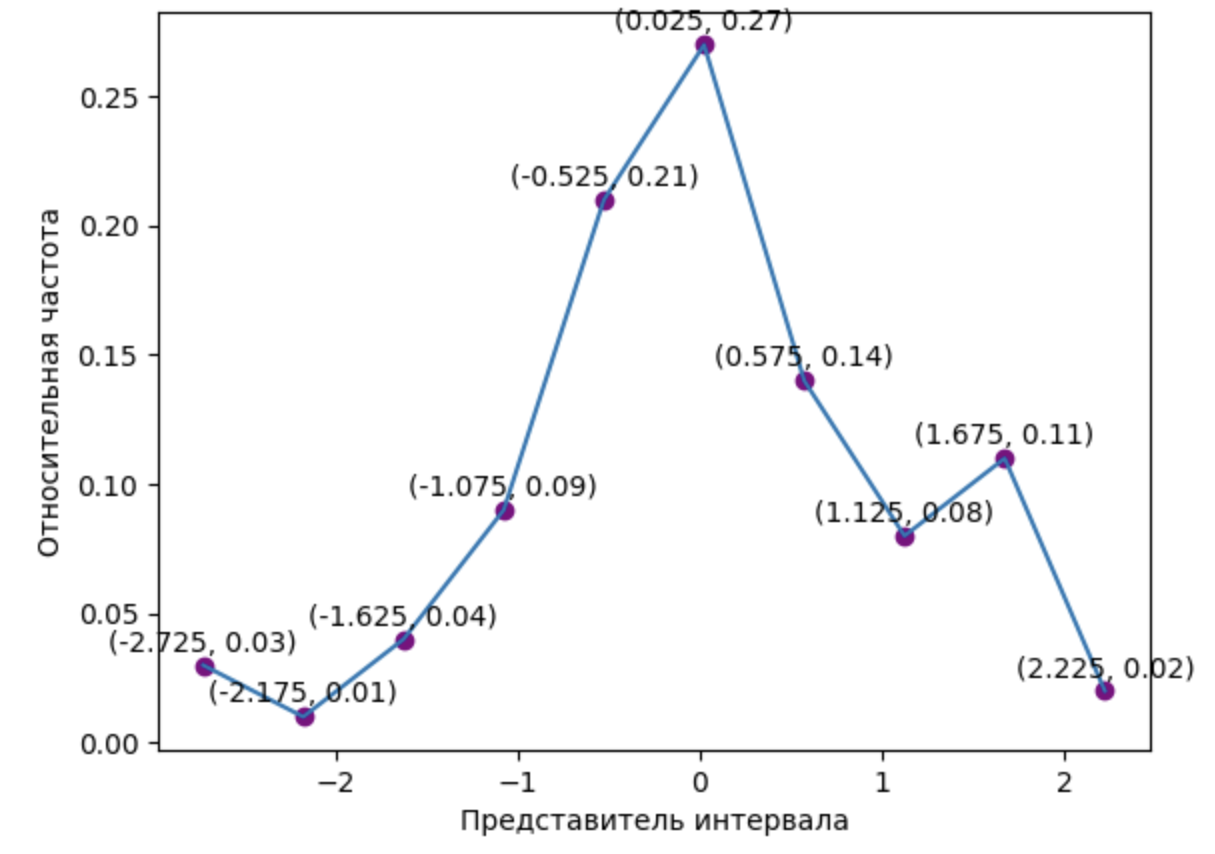
\includegraphics[width=.7\textwidth]{poligon.png}
\end{center} 

\begin{center}
    \small
    Рис.2 Полигон частот
\end{center} 
\newblock


\begin{center}
    \begin{figure}
        \centering
        \begin{tikzpicture}
        \begin{axis}[
            xlabel={$x$},
            ylabel={$F(x)$},
            ymin=0, ymax=1.1,
            xmin=-3.5, xmax=2.7,
            xtick={-3,-2.45,...,2.5},
            ytick={0,0.1,...,1},
            grid=both,
            width=12cm,
            height=8cm,
            legend style={at={(0.5,-0.15)},anchor=north},
            legend columns=-1,
            legend cell align=left,
            axis lines=middle, % <-- Вместо axis lines=box
        ]
        \addplot[const plot, mark=none, color=blue, dashed] coordinates {
                    (-3.5,0)
                    (-2.725, 0.03)
                    (-2.175, 0.04)
                    (-1.625, 0.08)
                    (-1.075, 0.17)
                    (-0.525, 0.38)
                    (0.025, 0.65)
                    (0.575, 0.79)
                    (1.125, 0.87)
                    (1.675, 0.98)
                    (2.225, 1)
                    (2.775, 1)
        };
        % Построение отрезков
        \draw[thick, black] (-3.5,0) -- (-2.725,0.0);
        \draw[thick, black] (-2.725,0.03) -- (-2.175,0.03);
        \draw[thick, black] (-2.175,0.04) -- (-1.625,0.04);
        \draw[thick, black] (-1.625,0.08) -- (-1.075,0.08);
        \draw[thick, black] (-1.075,0.17) -- (-0.525,0.17);
        \draw[thick, black] (-0.525,0.38) -- (0.025,0.38);
        \draw[thick, black] (0.025,0.65) -- (0.575,0.65);
        \draw[thick, black] (0.575,0.79) -- (1.125,0.79);
        \draw[thick, black] (1.125,0.87) -- (1.675,0.87);
        \draw[thick, black] (1.675,0.98) -- (2.225,0.98);
        \draw[thick, black] (2.225,1) -- (2.775,1);
        
        \end{axis}
        \end{tikzpicture}
        \caption{Эмпирическая функция}
        \label{fig:empirical_function}
        \end{figure}
\end{center}
\begin{center}
    \begin{figure}
        \centering
        \begin{tikzpicture}
        \begin{axis}[
            ybar interval,
            xlabel={Интервалы},
            ylabel={Высота столбцов},
            xtick=data,
            xticklabel style={rotate=45,anchor=east},
            xticklabels={[-3.0;-2.45),[-2.45;-1.9),[-1.9;-1.35),[-1.35;-0.8),[-0.8;-0.25),[-0.25;0.3),[0.3;0.85),[0.85;1.4),[1.4;1.95),[1.95;2.5],},
            ]
        \addplot+  coordinates {
                (-2.725, 0.05)
                (-2.175, 0.02)
                (-1.625, 0.07)
                (-1.075, 0.16)
                (-0.525, 0.38)
                (0.025, 0.49)
                (0.575, 0.25)
                (1.125, 0.15)
                (1.675, 0.2)
                (2.225, 0.04)
                (2.775, 0)
        };
        \end{axis}
        \end{tikzpicture}
        \caption*{Рис. 3 Гистограмма распределения}
    \end{figure}
\end{center}

\newblock
\section{Вычисление точечных оценок мат ожидания и дисперсии}
Найдем точечные оценки математического ожидания и дисперсии. В качестве таких оценок выбирают среднее выборочное значение:
\[\overline{X} = \sum_{i=1}^{10}x_i^*p_i^*\]
и выборочную дисперсию:
\[S^2 = \sum_{i=1}^{10}(x_i^* - \overline{X})^2p_i^* = \sum_{i=1}^{10}x_i^{*2}p_i^* - \overline{X}^2 = m_2 - \overline{X}^2\]
где 
\[m_2 = \sum_{i=1}^{10}x_i^{*2}p_i^*\]
\begin{table}[h]
    \begin{tabular}{|*{12}{c|}}
        \hline
        Номер & 1  & 2  & 3  & 4  & 5  & 6  & 7  & 8  & 9  & 10& некоторые рез-ты \\
        \hline
        $x_i^*$& -2.725 &-2.175 &-1.625 &-1.075 &-0.525 &0.025 &0.575 &1.125 &1.675 &2.225& -\\
        \hline
        $p_i^*$& 0.03 &0.01 &0.04 &0.09 &0.21 &0.27 &0.14 &0.08 &0.11 &0.02& -\\
        \hline
        $x_i^{*}p_i^*$& -0.082 &-0.022 &-0.065 &-0.097 &-0.11 &0.007 &0.081 &0.09 &0.184 &0.045& 0.011\\
        \hline
        $x_i^{*2}p_i^*$& 0.223 &0.047 &0.106 &0.104 &0.058 &0.0 &0.046 &0.101 &0.309 &0.099& 1.053\\
        \hline
    \end{tabular}
    \caption{Данные для подсчёта мат ожидания и дисперсии}
\end{table}
\\
Оценка математического ожидания: 0.011\\
Оценка дисперсии: 1.042 
\newblock
\section{Построить доверительные интервалы для мат ожидания и дисперсии}
Для рассматриваемого примера будем иметь:
\[\gamma = 0,95;\]
тогда находим по таблице распределения Стьюдента для 0.05 квантиль  t = 2.262, поэтому в нашем примере имеем:
\[\overline{X}-t\frac{S}{\sqrt{n}} = 0.011 - 2.262 \cdot\frac{\sqrt{1.042}}{\sqrt{10}} = -0.719\]
\[\overline{X}+t\frac{S}{\sqrt{n}} = 0.011 + 2.262 \cdot\frac{\sqrt{1.042}}{\sqrt{10}} = 0.741\]
таким образом:
\[-0.734 < m < 0.756\]
Для дисперсии определим квантили распределения хи-квадрат с 9 степенями свободы:
\[
\chi^2_{1-\alpha/2, n-1} = \chi^2_{1-\frac{0.05}{2}, 9} = \chi^2_{0.975, 9} = 2.7
\]
\[
\chi^2_{\alpha/2, n-1} = \chi^2_{0.025, 9} = 19.02
\]
По формуле подставим:
\[
\left(\frac{{(n-1)s^2}}{{\chi^2_{\alpha/2, n-1}}}, \frac{{(n-1)s^2}}{{\chi^2_{1-\alpha/2, n-1}}} \right)
\]
\[
\left( \frac{{9\cdot 1.042}}{19.02 }, \frac{{9\cdot 1.042}}{2.7} \right)
\]
Доверительный интервал для дисперсии:
\[ 0.493 < s^2 < 3.473\]
\section*{Вывод}
На основании анализа опытных данных: построили интервальный ряд; полигон частот; выборочную функцию распределения; гистограмму для изучения признака.
Вычислили точечные оценки мат ожидания и дисперсии.
Построили доверительные интервалы для мат ожидания и дисперсии с доверительной вероятностью 0,95.
\end{document}
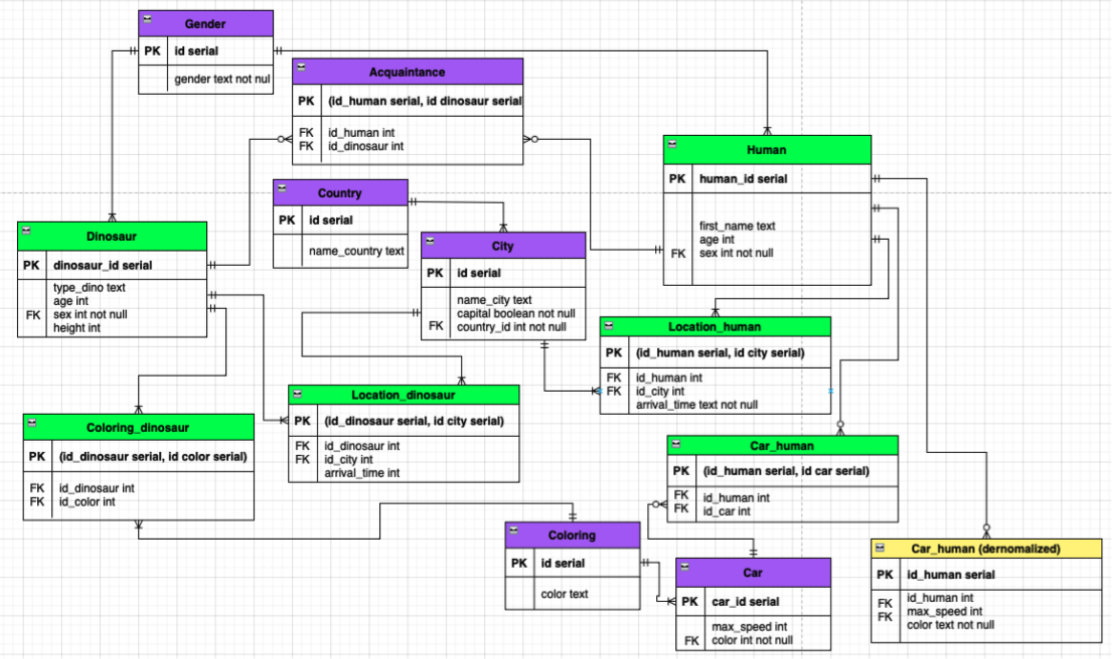
\includegraphics[width=.9\textwidth]{123}